\documentclass[a4paper, UTF8]{ctexbook}

\usepackage{amsmath}
\usepackage{amssymb}
\usepackage{amsthm}
\usepackage[dvipdfmx]{geometry}
\usepackage{graphicx}
\usepackage[toc]{multitoc}
\usepackage{paralist}
\usepackage{subcaption}
\usepackage{tabularx}
\usepackage{tcolorbox}
\usepackage{tkz-euclide}
\usepackage{wrapfig}
\usepackage{xcolor}
\usepackage[hidelinks]{hyperref}


\pagestyle{headings}

\makeatletter
\renewcommand\proofname{证明}
\renewenvironment{proof}[1][\proofname]{
	\par
	\pushQED{\qed}
	\normalfont\topsep6\p@\@plus6\p@\labelsep1em\relax
	\trivlist
	\item[\hskip\labelsep\indent\bfseries #1]\ignorespaces
}{
	\popQED\endtrivlist\@endpefalse
}
\makeatother
\newenvironment{desclist}{
	\begin{quote}\begin{compactdesc}
}{
	\end{compactdesc}\end{quote}
}
\newenvironment{enumlist}{
	\begin{quote}\begin{compactenum}
}{
	\end{compactenum}\end{quote}
}
\newenvironment{itemlist}{
	\begin{quote}\begin{compactitem}
}{
	\end{compactitem}\end{quote}
}
\newtheorem{example}{例}[section]

\title{{\Huge 高中数学笔记}}
\author{\textit{Jason Bowen Zheng}}

\begin{document}
\frontmatter
\maketitle
\section*{前言}
简而言之,该数学笔记整理了高中数学的所有知识点,供各位同学参考。它有点像教科书,但又不是教科书,这一点会在正文中慢慢体现出来。

这本笔记分成了如下部分:

\begin{description}
	\item[代数] 包括了高中代数这一纷繁杂乱的东西
	\item[函数] 涵盖了函数图像、单调性、对称性、周期性以及导数
	\item[三角学] 和三角比、三角函数以及三角形有关的东西
	\item[向量和复数] 向量和复数的相关知识
	\item[立体几何] 顾名思义,是三维的几何
	\item[计数原理] 排列组合和二项式的知识
	\item[概率和统计] 赌徒专用(雾)
\end{description}

该数学笔记亦提供了计算器的使用说明,适用于卡西欧\verb|fx-991CN X|。

同时,数学的学习不能局限于单一来源,我也会时不时附上一些清晰易懂的文章或视频的链接。

这本笔记是开源的,并且采用\href{https://creativecommons.org/licenses/by/4.0}{知识共享署名 4.0 国际许可协议}进行许可。您可以在\href{https://github.com/jason-bowen-zheng/math-notes}{这里}获取全部的源代码,亦可以提出改进意见。
\hypersetup{hidelinks}

\begin{flushright}
	\date{2022年11月}于上海
\end{flushright}

\tableofcontents
\clearpage
\mainmatter
\raggedbottom
\chapter{数理分析}
乍一看这个“数理分析”的标题感觉怪怪的,究竟什么是数理分析?在本章的最后有介绍,这是一种重要的数学思想。

在本章中,您将学会解不等式、求代数式的最值值域以及解方程。

\section{不等式}
在初中我们仅仅学了几种不等式的解法,这些很显然是不够的。在这里我们将学习更多的,以及奇奇怪怪的不等式的解法。

\subsection[有名]{有名不等式}
为了方便起见(真的吗?),我们把一些具有明显特征的不等式的集合称为\textbf{有名不等式}。解这些有名不等式必须按照既定的规则去解,否则就不对了。

\subsubsection{一元二次不等式}
如果您去翻一翻教科书,就会发现一元二次不等式的解法好复杂\footnote{这里参照的是沪教版的教科书。}。其实教科书仅仅把可能出现的结果罗列了一遍,并没有简化解法。

那现在重新定义一元二次不等式的解法:对于$ax^2+bx+c>0$且$a>0,\Delta>0$的情况下,大于为一元二次方程的两根之外;小于为两根之间。

\begin{example}
	解不等式$-x^2-5x-4\geq0$
\end{example}
\begin{proof}[解]
	由于二次项系数小于$0$,先变形:\[x^2+5x+4\leq0\]

	后解其对应的方程:\[x^2+5x+4=0\Rightarrow x_1=-4,x_2=-1\]

	转换为不等式的解集:\[x\in[-4,-1]\qedhere\]
\end{proof}

$\Delta\leq0$的情况太麻烦了,我们可以选择画出不等式对应二次函数的图像后再给出解集(无非就是一个解、$\mathbb{R}$或$\emptyset$)。

\subsubsection{分式不等式}
在初中我们也学习了分式方程的解法,千万不要和解分式不等式搞混了。

分式不等式的解法如下:

\begin{enumlist}
	\item 先移项、通分、化标,变为$\frac{x-a}{x-b}\gtrless0$
	\item 可将其看成解$(x-a)(x-b)\gtrless0$的问题
\end{enumlist}

若符号为$\leq$或$\geq$,将分母对应的根由闭变为开。

\subsubsection{绝对值不等式}

\subsubsection{最简指对不等式}
本小节介绍的是\textbf{最简}指对不等式的解法,即解它们的标准形式:\[a^x\gtrless b\text{和}\log_ax\gtrless b\]

\subsection[本质]{用本质解不等式}
在上一小节中我们学习了一些具有明显特征的不等式的解法,这仅仅是一半。接下来我们要面对的是一些奇奇怪怪的不等式。

\section{值域}
顾名思义,值域就是函数因变量(即$y$)的取值范围。

\subsection[本质]{本质(有图)}
一个函数有图像,画图然后在图上看出值域就行了:

\begin{enumlist}
\item 作图
\item 描深定义域
\item 根据定义域由下往上找到值域的范围
\end{enumlist}

\begin{example}
	求$y=x^2-2x, x\in(0,3)$的值域
\end{example}
\begin{proof}[解]
	先作如图\ref{fig:figure-of-a-function-and-its-domain}的函数图像\footnote{把求值域过程中的函数图像画出来就非常不好看,我们只画这一次。},描深定义域。

	\begin{figure}[htbp]
		\centering
		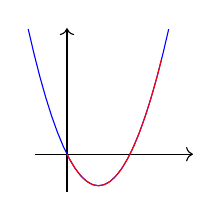
\begin{tikzpicture}[scale=0.4]
			\draw[->] (-1, 0) -- (4, 0);
			\draw[->] (0, -1.2) -- (0, 4);
			\draw[blue, domain=-1.23:3.23] plot(\x, \x * \x - 2 * \x);
			\draw[red, domain=0:3] plot(\x, \x * \x - 2 * \x);
		\end{tikzpicture}
		\caption{画图、描深}
		\label{fig:figure-of-a-function-and-its-domain}
	\end{figure}

	可得其最低点纵坐标为$-1$(是函数的顶点),两端点的纵坐标分别为$0$和$3$,故该函数值域为$[-1,3)$。
\end{proof}

\subsection[复合]{复合(无图)}
但是有些函数的图像你可是画不出来的,比如$y=4^x-2^{x+1}+1$。那就应该使用复合函数求值域的方法了。

如果一个函数$y=f(x)$可复合成$t=g(x)$和$y=f(t)$,那么可先求$g(x)$的值域,记为$A$。然后以$A$为定义域求$f(t)$的值域
(其中$f$、$g$均可作图)。

在第\ref{sec:mathsAnalysis-derivative-studyPorpertyOfFunction-figureOfFunction}节中,我们会了解到导数也可以用来求无图函数的值域。

\subsubsection{根式复合}
\subsubsection{分式复合}

\subsection{非复合}
上面介绍了这么多的复合函数求值域的方法,虽然多,但不可能用在所有函数上。那这些无法复合函数我们就不能求出它们的值域。

但是我们非常的幸运,拿到了一个单调函数(或者说函数在定义域内单调),那还是有办法的,直接代端点就可以了。

\begin{example}
	求$y=(\frac{1}{2})^x+(\frac{1}{3})^x,x\in(-\infty,2]$的值域
\end{example}
\begin{proof}[解]
	由题意得,函数单调递减。

	$\therefore y\in[\frac{13}{36},+\infty)$
\end{proof}

\section{何为数理分析}
在前面的小节中,我们学会了求解三样东西:不等式、值域和方程。它们是数理分析的主要手段。

数理分析的基本思想:等式(即方程)用掉一个等式,可以减少一个未知数的个数(即消元),最终获得只含一个未知数的等式、代数式或不等式。

所谓的数理分析即:在正式计算前的一种预测,即将多于等式的未知数全部用掉后,在最终一个等式的情况下,未知数还剩几个:

\begin{desclist}
	\item[若只剩一个未知数] 可求值
	\item[若剩两个未知数] 则可求范围
	\item[若剩超过两个未知数] 则此题还有变数(可能是条件还没有找到,可能需要等待一个巧合,可能是双变量等等)
\end{desclist}
\[\begin{aligned}
	\begin{cases}
		f(x,y,z)=0 \\
		g(x,y,z)=0 \\
		h(x,y,z)=0
	\end{cases}&\text{可分别解得$x,y,z$}
	&\begin{cases}
		f(x,y,z)=0 \\
		g(x,y,z)=0
	\end{cases}&\text{可求$x,y,z$的范围} \\
	\begin{cases}
		f(a,b,c,d)=0 \\
		g(a,b,c,d)=0
	\end{cases}&\text{未必可解}
	&\begin{cases}
		f(x)>0 \\
		g(x)>0
	\end{cases}&\text{分别解完后求交集} \\
	\begin{cases}
		f(x,y)>0 \\
		g(x,y)>0
	\end{cases}&\text{线性规划(同向可加)}
	&\begin{cases}
		f(x,y)>0 \\
		g(x,y)=0
	\end{cases}&\text{利用$g$消元,可解$f$}
\end{aligned}\]

注意可解不等式只能含一个变量,不等式组也只能含一个变量,不等式组只是解集的交并关系,不等式不可用来消元。

多变量不等式是线性规划问题(同向可加性是最简线性规划问题)。

在有多个字母的情况下(尤其是涉及到复数),使用数理分析可快速的找到解题思路。

\chapter{函数性质}
函数能够很好的描述一样东西的变化规律,从而得出结论(从先前章节的笔记就可以看出)。但这还不够,想要深入分析,我们还是要了解更多的知识。

在本章中,你会学习一些新的函数及其图像。再依靠图像,得出函数的某些性质,并证明之。

\section{函数图像}
在初中我们学过一次函数、反比例函数以及二次函数,它们的图像就不再介绍了。如记性不好的去请教初中数学老师。

顺带提一句:下文讲述的函数的绘制方法只能画出近似的、粗略的函数图像,这种精度在绝大多数情况下是没有问题的\footnote{例外情况指方程的解的个数问题,前文已经提过。},您也应该在绝大多数情况下绘制这种图像。

对于三角函数,会在后面的“三角函数”章节提到。这里仅仅画出它们的图像而不研究其性质。

\subsection{耐克函数}
首先介绍的是耐克函数(或称对勾函数),它的解析式形如:\[y=ax+\frac{b}{x}\]

通过描点法,不难画出它的图像(如图\ref{fig:figure-of-tick-functions})。

\begin{figure}[htb]
	\centering
	\begin{subfigure}[b]{0.24\textwidth}
		\centering
		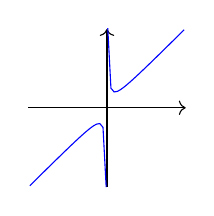
\begin{tikzpicture}[scale=0.1]
			\draw[->] (-10, 0) -- (10, 0);
			\draw[->] (0, -10) -- (0, 10);
			\draw[color=blue, domain=0.1:9.8] plot(\x, \x + 1 / \x);
			\draw[color=blue, domain=-9.8:-0.1] plot(\x, \x + 1 / \x);
		\end{tikzpicture}
		\caption{$y=1+\frac{1}{x}$}
		\label{fig:figure-of-tick-functions-a}
	\end{subfigure}
	\begin{subfigure}[b]{0.24\textwidth}
		\centering
		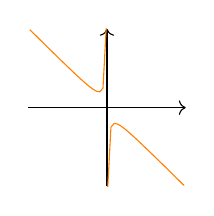
\begin{tikzpicture}[scale=0.1]
			\draw[->] (-10, 0) -- (10, 0);
			\draw[->] (0, -10) -- (0, 10);
			\draw[color=orange, domain=0.1:9.8] plot(\x, -\x - 1 / \x);
			\draw[color=orange, domain=-9.8:-0.1] plot(\x, -\x - 1 / \x);
		\end{tikzpicture}
		\caption{$y=-1-\frac{1}{x}$}
		\label{fig:figure-of-tick-functions-b}
	\end{subfigure}
	\begin{subfigure}[b]{0.24\textwidth}
		\centering
		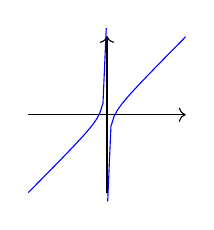
\begin{tikzpicture}[scale=0.1]
			\draw[->] (-10, 0) -- (10, 0);
			\draw[->] (0, -10) -- (0, 10);
			\draw[color=blue, domain=0.09:10] plot(\x, \x - 1 / \x);
			\draw[color=blue, domain=-10:-0.09] plot(\x, \x - 1 / \x);
		\end{tikzpicture}
		\caption{$y=1-\frac{1}{x}$}
		\label{fig:figure-of-tick-functions-c}
	\end{subfigure}
	\begin{subfigure}[b]{0.24\textwidth}
		\centering
		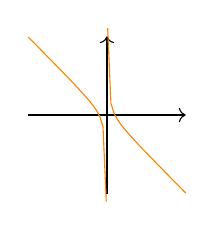
\begin{tikzpicture}[scale=0.1]
			\draw[->] (-10, 0) -- (10, 0);
			\draw[->] (0, -10) -- (0, 10);
			\draw[color=orange, domain=0.09:10] plot(\x, -\x + 1 / \x);
			\draw[color=orange, domain=-10:-0.09] plot(\x, -\x + 1 / \x);
		\end{tikzpicture}
		\caption{$y=-1+\frac{1}{x}$}
		\label{fig:figure-of-tick-functions-d}
	\end{subfigure}
	\caption{参量取不同值时耐克函数的图像}
	\label{fig:figure-of-tick-functions}
\end{figure}

然后我们可以得出耐克函数图像的性质:

\begin{itemlist}
	\item $a^+,b^+$是一、三象限的耐克函数(如图\ref{fig:figure-of-tick-functions-a})
	\item $a^-,b^-$是二、四象限的耐克函数(如图\ref{fig:figure-of-tick-functions-b})
	\item $a^+,b^-$是双增函数(如图\ref{fig:figure-of-tick-functions-c})
	\item $a^-,b^+$是双减函数(如图\ref{fig:figure-of-tick-functions-d})
\end{itemlist}

再看一眼函数图像,$a$、$b$同号时在各个象限内有极值点,接下来将推导出这个点的坐标:

\begin{proof}
	根据基本不等式得:\[ax+\frac{b}{x}\geq2\sqrt{ab}\]

	此时不等号右边即极值点的纵坐标,代入原式解方程:
	\[\begin{split}
		&ax+\frac{b}{x}=2\sqrt{ab} \\
		&ax^2-2x\sqrt{ab}+b=0 \\
		&x=\sqrt{\frac{b}{a}}
	\end{split}\]

	可以得到耐克函数在第一象限内的顶点坐标为$(\sqrt{\frac{b}{a}},2\sqrt{ab})$,其它象限只需在对应的地方添负号即可。
\end{proof}

\subsection{幂函数}
在初中我们学过了反比例函数、二次函数,它们都是幂函数的一种。其解析式为:\[y=x^a(a=\frac{p}{q}\quad p,q\in\mathbb{Z})\]

要绘制幂函数的图像,应把第一象限的图像和其余部分的图像分别绘制。

第一象限的图像如图\ref{fig:figure-of-power-function}所示。

\begin{figure}[htb]
	\centering
	\begin{subfigure}[b]{0.3\textwidth}
		\centering
		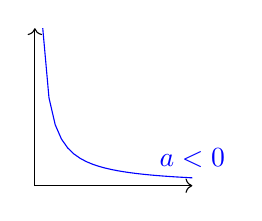
\begin{tikzpicture}[scale=0.2]
			\draw[->] (0, 0) -- (10, 0);
			\draw[->] (0, 0) -- (0, 10);
			\draw[color=blue, domain=0.5:10] plot(\x, 5 / \x) node[above] {$a<0$};
		\end{tikzpicture}
		\caption{减}
	\end{subfigure}
	\begin{subfigure}[b]{0.3\textwidth}
		\centering
		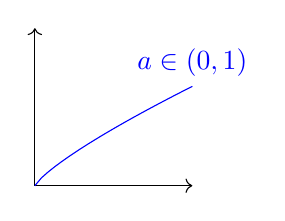
\begin{tikzpicture}[scale=0.2]
			\draw[->] (0, 0) -- (10, 0);
			\draw[->] (0, 0) -- (0, 10);
			\draw[color=blue, domain=0:10] plot(\x, \x ^ 0.8) node[above] {$a\in(0,1)$};
		\end{tikzpicture}
		\caption{缓慢增}
	\end{subfigure}
	\begin{subfigure}[b]{0.3\textwidth}
		\centering
		\begin{tikzpicture}[scale=0.2]
			\draw[->] (0, 0) -- (10, 0);
			\draw[->] (0, 0) -- (0, 10);
			\draw[color=blue, domain=0:6.81] plot(\x, \x ^ 1.2) node[right] {$a>1$};
		\end{tikzpicture}
		\caption{快速增}
	\end{subfigure}
	\caption{幂函数第一象限内的图像}
	\label{fig:figure-of-power-function}
\end{figure}

其它象限的图像可按照下面的流程绘出:
\[\begin{cases}
	\text{$q$为偶数} & \text{只有第一象限图像} \\
	\text{$q$为奇数} & \text{判断$p$}
	\begin{cases}
		\text{$p$为奇数} & \text{函数为奇函数} \\
		\text{$p$为偶数} & \text{函数为偶函数}
	\end{cases}
\end{cases}\]

\section{反函数}
我们知道,将某一个特定的值代入函数的自变量(即$x$)可以求出因变量(即$y$)的值。那已知$y$求$x$呢?解方程即可。

那我们就可以更进一步,直接用$y$来表示$x$,那就是\textbf{反函数}了。

由于函数需要$x$对应一个$y$,所以我们可以得到$x$、$y$\textbf{一一对应}是反函数存在的充要条件。

\chapter{导数}
在此首先恭喜您,当看到“导数”这个词时,阁下即将面对的是数学的一个全新的分支---\textbf{微积分学}(calculus)。简而言之,它将我们研究函数的视角从宏观拓展到了微观。

听起来似乎很难,不过这只是高中难度的知识,我们也只学习导数及其应用,也没这么难吧(应该)。

YouTube频道3Blue1Brown有10部讲述“微积分的本质”的视频,我会按学习进度推荐您看其中的6部。

\section{概念}
有一描述直线的函数$f(x)=2x$,当问及“$x=1$时函数的斜率是多少”,您一定会说是2。这很简单,因为$f(x)$的斜率处处相等。

那请问当$x=1$时,$f(x)=x^2$的斜率为多少呢?

作为一个不知道微积分为何物的高中生,您决定试一试,透过斜率的定义\footnote{简单来说,斜率$k=\dfrac{\Delta y}{\Delta x}$,即垂直方向的变化量与水平方向的变化量的比值。}来解决这个问题。

\begin{figure}[htb]
    \centering
    \begin{asy}
        import graph;
        write("asy: Generating 'fig:calc-slope'");

        size(4cm, 4cm);

        real f(real x){return x^2;}
        real fp(real x){return 2.5*x-1.5;}

        draw(graph(f, -2, 2), red);
        draw(graph(fp, 0, 2), blue);
        xaxis("$x$", EndArrow);
        yaxis("$y$", EndArrow);

        draw((1, 1) -- (1.5, 1), L=scale(0.5)*Label("$\Delta x$", position=MidPoint));
        draw((1.5, 1) -- (1.5, 1.5^2), L=scale(0.5)*Label("$\Delta y$", position=MidPoint));
        dot((1, 1), L=scale(0.5)*Label("$A$", align=NW));
        dot((1.5, 1.5^2), L=scale(0.5)*Label("$B$", align=W));
    \end{asy}
    \caption{计算二次函数的斜率}
    \label{fig:calc-slope}
\end{figure}

您或许会画出如图\ref{fig:calc-slope}所示的函数图像,那接下来我们就可以使用由两条直角边$\Delta x$和$\Delta y$组成的直角三角形来计算斜率。

二次函数上$A$点处的斜率是我们要求的,我们可以让抛物线上的$B$点慢慢靠近$A$点,这样直角三角形会越来越小,结果也会变得精确。我们就可以写出式子\eqref{equ:calc-slope}来表示斜率
\begin{gather}
    k=\frac{(1+\Delta x)^2-1^2}{\Delta x} \label{equ:calc-slope}
\end{gather}

给$\Delta x$多次赋值,我们不难发现最后它会收敛到2,由此可知$f(x)=x^2$在$x=1$处的斜率是2。
\begin{align*}
    \Delta x=0.1\quad & k=2.1 \\
    \Delta x=0.01\quad & k=2.01 \\
    \Delta x=0.001\quad & k=2.001 \\
\end{align*}

好,我们算完了,感觉很简单吧!\textbf{导数}(derivative)就是这样,研究函数在某一点附近的变化率。我们刚刚寻找函数某点导数的过程称为\textbf{求导}(differentiation)。

同时,为了避免每次求导都要考虑函数图像,求$f(x)$在$x=x_0$处的导数$f'(x_0)$有公式\[f'(x_0)=\lim_{h\to0}\frac{f(x_0+h)-f(x_0)}{h}\]这和我们刚刚得到的式子\eqref{equ:calc-slope}很像,只不过我们使用了极限的表示方法。

% TODO: \section{公式}
% TODO: \section{运用}


\chapter{立体几何}
我们在初中时期学习了平面几何,研究了平面上一些简单图形及其几何性质;在高中时期,我们也通过三角比及三角函数对三角形有了更深入的理解。现在,我们将增加一个纬度,研究三维空间中的几何体的性质。与其它高中的知识相比较,甚至是与初中的平面几何比较,立体几何都是简单的:它更注重于计算,而非证明,也不需要苦思冥想如何添辅助线。那么,放松,进入立体几何的世界吧!

\end{document}
